\documentclass[,hyphens]{sigchi}

% Use this section to set the ACM copyright statement (e.g. for
% preprints).  Consult the conference website for the camera-ready
% copyright statement.

% Copyright
\CopyrightYear{2020}
%\setcopyright{acmcopyright}
\setcopyright{acmlicensed}
%\setcopyright{rightsretained}
%\setcopyright{usgov}
%\setcopyright{usgovmixed}
%\setcopyright{cagov}
%\setcopyright{cagovmixed}
% DOI
\doi{https://doi.org/10.1145/3313831.XXXXXXX}
% ISBN
\isbn{978-1-4503-6708-0/20/04}
%Conference
\conferenceinfo{CHI'20,}{April  25--30, 2020, Honolulu, HI, USA}
%Price
\acmPrice{\$15.00}

% Use this command to override the default ACM copyright statement
% (e.g. for preprints).  Consult the conference website for the
% camera-ready copyright statement.

%% HOW TO OVERRIDE THE DEFAULT COPYRIGHT STRIP --
%% Please note you need to make sure the copy for your specific
%% license is used here!
% \toappear{
% Permission to make digital or hard copies of all or part of this work
% for personal or classroom use is granted without fee provided that
% copies are not made or distributed for profit or commercial advantage
% and that copies bear this notice and the full citation on the first
% page. Copyrights for components of this work owned by others than ACM
% must be honored. Abstracting with credit is permitted. To copy
% otherwise, or republish, to post on servers or to redistribute to
% lists, requires prior specific permission and/or a fee. Request
% permissions from \href{mailto:Permissions@acm.org}{Permissions@acm.org}. \\
% \emph{CHI '16},  May 07--12, 2016, San Jose, CA, USA \\
% ACM xxx-x-xxxx-xxxx-x/xx/xx\ldots \$15.00 \\
% DOI: \url{http://dx.doi.org/xx.xxxx/xxxxxxx.xxxxxxx}
% }

% Arabic page numbers for submission.  Remove this line to eliminate
% page numbers for the camera ready copy
\pagenumbering{arabic}

% Load basic packages
\usepackage{balance}       % to better equalize the last page
\usepackage{graphics}      % for EPS, load graphicx instead 
\usepackage[T1]{fontenc}   % for umlauts and other diaeresis
\usepackage{txfonts}
\usepackage{mathptmx}
\usepackage[pdflang={en-US},pdftex]{hyperref}
\usepackage{color}
\usepackage{booktabs}
\usepackage{textcomp}

% Some optional stuff you might like/need.
\usepackage{microtype}        % Improved Tracking and Kerning
% \usepackage[all]{hypcap}    % Fixes bug in hyperref caption linking
\usepackage{ccicons}          % Cite your images correctly!
% \usepackage[utf8]{inputenc} % for a UTF8 editor only

% If you want to use todo notes, marginpars etc. during creation of
% your draft document, you have to enable the "chi_draft" option for
% the document class. To do this, change the very first line to:
% "\documentclass[chi_draft]{sigchi}". You can then place todo notes
% by using the "\todo{...}"  command. Make sure to disable the draft
% option again before submitting your final document.
\usepackage{todonotes}

% Paper metadata (use plain text, for PDF inclusion and later
% re-using, if desired).  Use \emtpyauthor when submitting for review
% so you remain anonymous.
\def\plaintitle{SIGCHI Conference Proceedings Format}
\def\plainauthor{First Author, Second Author, Third Author,
  Fourth Author, Fifth Author, Sixth Author}
\def\emptyauthor{}
\def\plainkeywords{Authors' choice; of terms; separated; by
  semicolons; include commas, within terms only; this section is required.}
\def\plaingeneralterms{Documentation, Standardization}

% llt: Define a global style for URLs, rather that the default one
\makeatletter
\def\url@leostyle{%
  \@ifundefined{selectfont}{
    \def\UrlFont{\sf}
  }{
    \def\UrlFont{\small\bf\ttfamily}
  }}
\makeatother
\urlstyle{leo}

% To make various LaTeX processors do the right thing with page size.
\def\pprw{8.5in}
\def\pprh{11in}
\special{papersize=\pprw,\pprh}
\setlength{\paperwidth}{\pprw}
\setlength{\paperheight}{\pprh}
\setlength{\pdfpagewidth}{\pprw}
\setlength{\pdfpageheight}{\pprh}

% Make sure hyperref comes last of your loaded packages, to give it a
% fighting chance of not being over-written, since its job is to
% redefine many LaTeX commands.
\definecolor{linkColor}{RGB}{6,125,233}
\hypersetup{%
  pdftitle={\plaintitle},
% Use \plainauthor for final version.
%  pdfauthor={\plainauthor},
  pdfauthor={\emptyauthor},
  pdfkeywords={\plainkeywords},
  pdfdisplaydoctitle=true, % For Accessibility
  bookmarksnumbered,
  pdfstartview={FitH},
  colorlinks,
  citecolor=black,
  filecolor=black,
  linkcolor=black,
  urlcolor=linkColor,
  breaklinks=true,
  hypertexnames=false
}

% create a shortcut to typeset table headings
% \newcommand\tabhead[1]{\small\textbf{#1}}

% End of preamble. Here it comes the document.
\begin{document}

\title{We are the Greatest Showmen: Configuring Mobile Learning Technologies for Student-Led Activities}

\numberofauthors{3}
\author{%
  \alignauthor{Leave Authors Anonymous\\
    \affaddr{for Submission}\\
    \affaddr{City, Country}\\
    \email{e-mail address}}\\
  \alignauthor{Leave Authors Anonymous\\
    \affaddr{for Submission}\\
    \affaddr{City, Country}\\
    \email{e-mail address}}\\
  \alignauthor{Leave Authors Anonymous\\
    \affaddr{for Submission}\\
    \affaddr{City, Country}\\
    \email{e-mail address}}\\
}

\maketitle

\begin{abstract}
While the use of mobile learning technologies by teachers and community experts has been explored by HCI research, little attention has been given to how they could enhance learning activities designed by the students themselves. Following an action research approach, we report on engagements inside and outside of the classroom with both teachers and students from three different UK schools, using a variety of configurations to work within given time constraints and produce student-led mobile learning activities using the OurPlace application. We also report on the use of the OurPlace to facilitate an exchange of knowledge and values between a class from an ethnically diverse inner-city school and the children of a community of travelling Showmen. We contribute insights gained from these studies, and offer suggestions for how project-based mobile learning technologies can be better configured within the restrictions of a formal education environment to support student independence, heritage learning and the exchanging of values.
\end{abstract}


% ACM Classfication

\begin{CCSXML}
<ccs2012>
<concept>
<concept_id>10003120.10003121</concept_id>
<concept_desc>Human-centered computing~Human computer interaction (HCI)</concept_desc>
<concept_significance>500</concept_significance>
</concept>
<concept>
<concept_id>10003120.10003121.10003125.10011752</concept_id>
<concept_desc>Human-centered computing~Haptic devices</concept_desc>
<concept_significance>300</concept_significance>
</concept>
<concept>
<concept_id>10003120.10003121.10003122.10003334</concept_id>
<concept_desc>Human-centered computing~User studies</concept_desc>
<concept_significance>100</concept_significance>
</concept>
</ccs2012>
\end{CCSXML}

\ccsdesc[500]{Human-centered computing~Human computer interaction (HCI)}
\ccsdesc[300]{Human-centered computing~Haptic devices}
\ccsdesc[100]{Human-centered computing~User studies}

% Author Keywords
\keywords{\plainkeywords}

% Print the classification codes
\printccsdesc
Please use the 2012 Classifiers and see this link to embed them in the text: \url{https://dl.acm.org/ccs/ccs_flat.cfm}



\section{Introduction}

Introduce context school pressures, limitations
Rising role of mobile technology

\section{Related Work}

\subsection{Constructionism}
The learning theory of constructionism, introduced by Seymour Papert in the mid-1980s, argues that constructing, sharing and reflecting upon physical or virtual `public entities' can be a powerful way for learners to build `knowledge structures'--collections of knowledge, concepts and facts interrelated through various semantic relationships \cite{PapertSeymourandHarel1991a}. Papert argues that the process of learning is the building of these knowledge structures, a process which--while it occurs irrespective of the circumstances of the learning--happens `\textit{especially felicitously in a context where the learner is consciously engaged in constructing a public entity}'. These public entities could range from physical artefacts such as models of buildings, virtual programming code or even conceptual theories of the universe. In their overview of constructionism, Noss and Hoyles use Logo (a simple programming environment which included a `turtle' entity, whose movements around the screen could be programmed \cite{Harvey1997}) as an example of a constructionist working environment \cite{Noss2017}. They argue that this environment offered a medium in which learners could `\textit{explore and learn from feedback, much as one can master a foreign language by living in the appropriate country}'. Noss and Hoyles also claim that Logo's environment affords learners to take ownership of a construction-based approach, potentially leading to greater engagement, confidence and empowerment. Finally, they posit that through exploration and construction of public entities, learners can encounter `powerful ideas': `\textit{concepts and strategies  that confront and build upon intuitive knowledge}'. For this reason, Noss and Hoyles argue that constructionist tools need to be expressive enough to facilitate these ideas emerging through the learner's construction of public entities.

\subsection{Project-Based Learning}
Blumenfeld et al note that small, easily assessed tasks which focus on low-level facts and skills (e.g. tasks commonly found on worksheets) have become the focus of American classrooms \cite{Blumenfeld1991}. However, they argue that these tasks afford students `\textit{few opportunities to represent knowledge in a variety of ways, pose and solve real problems, or use their knowledge to create artifacts}'. They argue that a preferable alternative is project-based learning (PBL), which they describe as an approach to teaching and learning which focuses on engaging students through the investigation of non-trivial, `authentic' problems in a manner which supports learner autonomy over the course of an extended project. Frequently, these projects will result in the creation of an artifact in response to a given question or problem (such as videos, reports, artworks, websites or performances \cite{Holubova2008}), in effect making PBL a method of applying constructionism in response to real-world problems and supporting the inclusion of prior knowledge, domain research and greater levels of student autonomy. Previous research has argued that these projects can serve to build bridges between classroom activities and real-life experiences \cite{Blumenfeld1991}, enhance applied and conceptual knowledge around a subject \cite{Boaler1999}, and that PBL's greater levels of autonomy and challenge can result in higher levels of student engagement \cite{Wurdinger2007}.

Project-based learning is also recognised as fertile ground for technology-enhanced learning. Bell argues that `\textit{technology as a means, not an end, enables students to experiment with different technologies for all aspects of PBL}' (including research and data collection, knowledge sharing and artifact creation) and that it can be `\textit{highly engaging to students, because it taps into their fluency with computers}' \cite{Bell2010}. ChanLin describes how students used digital technologies within PBL for researching on the web, taking photographs, participating in online communities and creating web pages as final artifacts \cite{ChanLin2008}. Krajcik et al note that while the use of mobile and desktop technologies help students build knowledge structures and form deeper and richer understandings of the subjects at hand, teachers frequently run into challenges in gaining access to computing hardware due to multiple classes sharing resources \cite{Krajcik2006}.

While some studies have found that project-based instruction is not necessarily more demanding in terms of teaching time and resources \cite{Al-Balushi2014}, Blumenfeld et al posit that by its nature PBL `\textit{requires active engagement of students' effort over an extended period of time}' \cite{Blumenfeld1991}. Krajcik et al argue that `\textit{it takes more time to complete a task where students are constructing their own knowledge in meaningful, situated activities}', leading to teachers being hesitant to put it into practice when faced with strict and competing curriculum goals \cite{Krajcik2006}. The non-profit organisation Innovation Unit note `\textit{[PBL] can be a powerful learning strategy if it is part of a whole school change process, and [schools] are ready and able to make the necessary time and staff available}' \cite{InnovationUnit2016}, suggesting that putting PBL into practice requires substantial changes in how teachers approach classroom structures, activities and tasks. This is easier said than done, particularly when teachers and schools work within structures which pressure them to conform to quantifiable testing methods, propagating the aforementioned worksheet-style tasks and `teaching to the test'. For example, the head of the UK's Office for Standards in Education (Ofsted) has noted that `\textit{[Ofsted] have created a situation where second-guessing the test can trump the pursuit of real, deep knowledge and understanding}' \cite{Ofsted2018}. All of these factors result in varying levels of restrictions placed upon teachers, impacting their time affordances, curriculum content and pedagogical approaches. This has meant that  implementing project-based learning in UK schools has proven to be a challenge \cite{TheEducationEndowmentFoundation2016}.

\subsection{The TPACK Framework}

The Technological Pedagogical Content Knowledge framework (TPACK, Figure~\ref{fig:TPACK}) provides a model which describes the roles of and interactions between what Koehler and Mishra argue are the three main components of teachers' knowledge: content, pedagogy and technology \cite{Harris2009}. In the model, content knowledge refers to the teacher's knowledge about the domain and subject matter to be learned or taught; technological knowledge refers to an evolving understanding of how technology could assist or impede the achievement of a goal; and pedagogical knowledge is the teacher's understanding of the processes, practices and methods of teaching and learning. Furthermore, each of these interact with each other (for example, technological pedagogical knowledge describes an understanding of how teaching and learning can change when technologies are used in different ways), and exist within diverse contexts (e.g. environmental, socioeconomic). 

\begin{figure}
\centering
  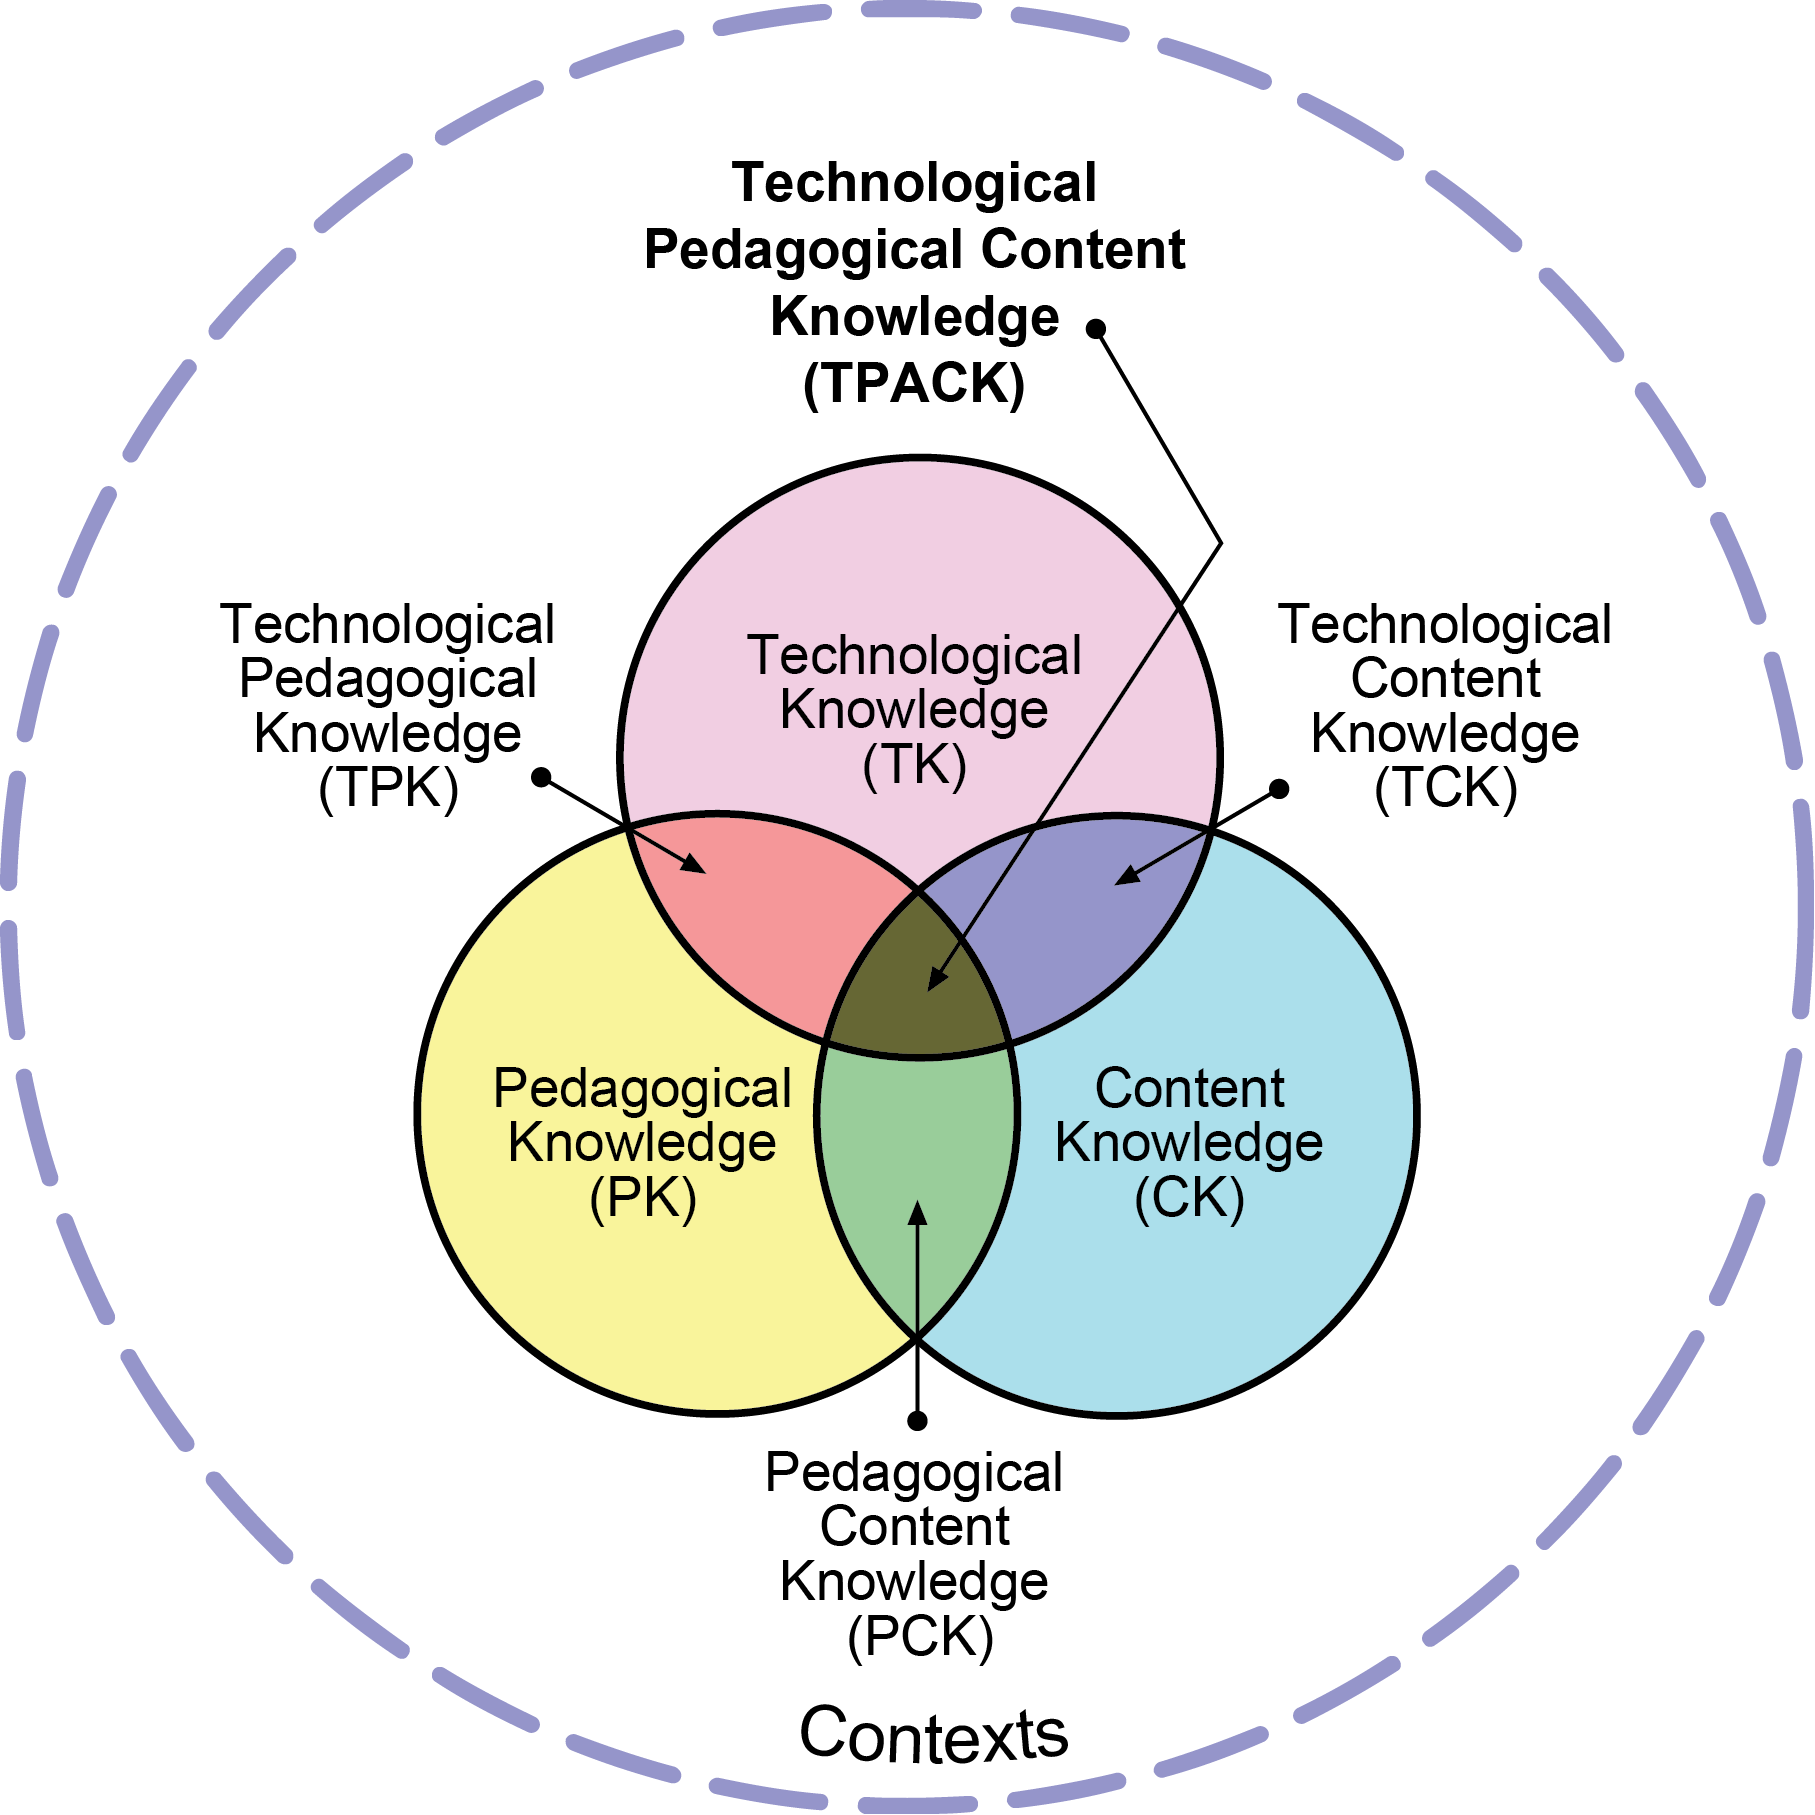
\includegraphics[width=0.9\columnwidth]{figures/TPACK-new}
  \caption{The TPACK model of teacher knowledge, which shows the interactions between teachers' knowledge of technology, pedagogy and content across different teaching contexts.}~\label{fig:TPACK}
\end{figure}

Koehler and Mishra argue that when taken as a whole, the TPACK framework describes `\textit{the basis for effective teaching with technology}', including how technologies can be used effectively within the teaching process for representing new concepts and building upon existing student knowledge. They also posit that any changes in one of the three main components has to be `compensated' by changes to the other two. They note that this is frequently seen with technology, as it can be rapidly evolving, opaque in its inner-workings and multi-purpose. One given example is the increasing usage of the Internet for online learning, which forced educators to think about how educational content can be represented in new ways on the web, and how it can be used to connect students to content, communities and each other.  The authors argue that the model discourages teachers and researchers from `\textit{oversimplified approaches which treat technology as an add-on'}, and instead regarding teachers' technology knowledge as being in a dynamic equilibrium with content and pedagogical knowledge.

\subsection{Mobile Learning}

Mobile learning (`\textit{learning across multiple contexts, through social and content interactions using personal electronic devices}' \cite{Crompton2013}, AKA `m-learning') has continued to play a large role within schools in the UK, with ready access to tablet computers becoming more common in schools (44\% of UK schools are expected to have one tablet per child by 2020 \cite{BritishEducationalSuppliersAssociation2015}), and their general ubiquity meaning most of the younger population is familiar with their use (87\% of UK adults report owning a smartphone \cite{Statistica2018}, as do 84\% of children aged between 8-16 \cite{Statistica2018a}). While traditional desktop and laptop devices are currently still more common in schools (numbering approximately 3.4 million in 2017 \cite{BritishEducationalSuppliersAssociation2017}), mobile devices have been touted as having a number of advantages over their more stationary counterparts: for example, Traxler argues that mobile technologies can offer structured educational experiences which can be situated in--and responsive to--authentic learning environments \cite{Traxler2011}. This makes m-learning a potentially great fit for subscribers to Lave and Wenger's Situated Learning Theory, which posits that learning unintentionally occurs in authentic activities, contexts and cultures through `legitimate participation' in communities of practice \cite{Lave1991}. Sharples et al argue that to better utilise these advantages, m-learning technologies should take into account the physical and social aspects of the learning context (both physical and social); the amount of control the learner has over the activity; and the learner's communication with others \cite{Sharples2007}.

research where mobile tech has been used in project based learning

Previous m-learning research has used these capabilities for a wide variety of applications, such as sensing tool kits to conduct citizen science \cite{Sharples2017}; enabling seamless learning across classrooms and museums on school trips \cite{Vavoula2009}; and empowering children in collecting evidence to support their advocacy and engagement in urban design processes \cite{Peacock2018}. Prior research has also shown that m-learning technologies can enhance the development of relationships with place, and act as a medium through which stakeholders can harness the underlying socioeconomic infrastructures of place as learning resources \cite{Richardson2017}. In the ParkLearn project, Richardson et al attempted to combine elements of all of the above into a single mobile application supporting creating, sharing and engaging with bespoke, place-based m-learning activities `\textit{that leverage the targeted learning environment and mobile devices' hardware to support situated learning}' \cite{Richardson2018}. Through using ParkLearn in longitudinal studies with a primary school and volunteers at a local park, the authors found that the app promoted a sense of ownership in both learners and activity creators by supporting greater degrees of creativity and independence. Furthermore, the app was shown to be an effective medium through which physical and social aspects of the local environment could be leveraged as learning resources.

summary - motivation for using the ourplace app in a project-based learning context, exploring different configurations of curricula

\section{The OurPlace App}

OurPlace is the current iteration of the open-source ParkLearn platform, with an expanded feature set and re-branded to support its use in contexts outside of local parks \cite{Richardson2018a}. Consisting of a website and mobile applications for both Android and iOS, OurPlace supports the creation, sharing and engagement with with m-learning activities (`Activities'), each of which is built up from smaller, modular tasks (`Tasks'). These tasks each consist of a specific interaction (`Task Type'), which either promote creativity, emulate traditional classroom learning materials or use the device's hardware to give context-specific experiences (Table~\ref{tab:TaskTypes}). With the exception of \textit{Scan the QR Code}, all of these Task Types were present in the original ParkLearn application. An Activity can have any number of Tasks within it. OurPlace also adds support for `Follow-Up Tasks', which allow activity creators to add sub-tasks which unlock once their parent task has been completed (Figure~\ref{fig:ActivityCreation}.e). This supports the design of more complicated combinations of interactions (for example: a \textit{Location Hunt} could unlock a \textit{Record Audio} and \textit{Take a Photo} once the user arrives at a designated location, or a \textit{Multiple Choice} could quiz the user about what they've just heard in a \textit{Listen to Audio}).

\begin{table}
  \centering
  \begin{tabular}{l|p{50mm}}
    % \toprule
    {\small\textit{Task Type}}
    & {\small \textit{Interaction Description}} \\
    \midrule
    Information & Read some written information, with an optional accompanying image and hyperlink to an external web page \\
    Listen to Audio & Listen to a given audio recording \\
    Take a Photo & Use the camera to take still images in response to an instruction \\
    Photo Match & Use the camera to match an existing photo given as an overlay \\
    Draw a Picture & Draw a picture onto a blank canvas \\
    Draw on Photo & Draw on top of a given image \\
    Record Video & Record a video using the camera \\
    Record Audio & Record an audio clip using the device's microphone \\
    Map Marking & Mark a given number of locations onto a Google Map \\
    Location Hunt & Track down a target location by observing your reported distance from it \\
    Scan the QR Code & Find and scan the correct QR code \\
    Multiple Choice & Choose a response from a set of text options \\
    Text Entry & Enter a response using the device's keyboard
    % \bottomrule
  \end{tabular}
  \caption{The Task Types available in the OurPlace application}~\label{tab:TaskTypes}
\end{table}

\begin{figure*}
  \centering
  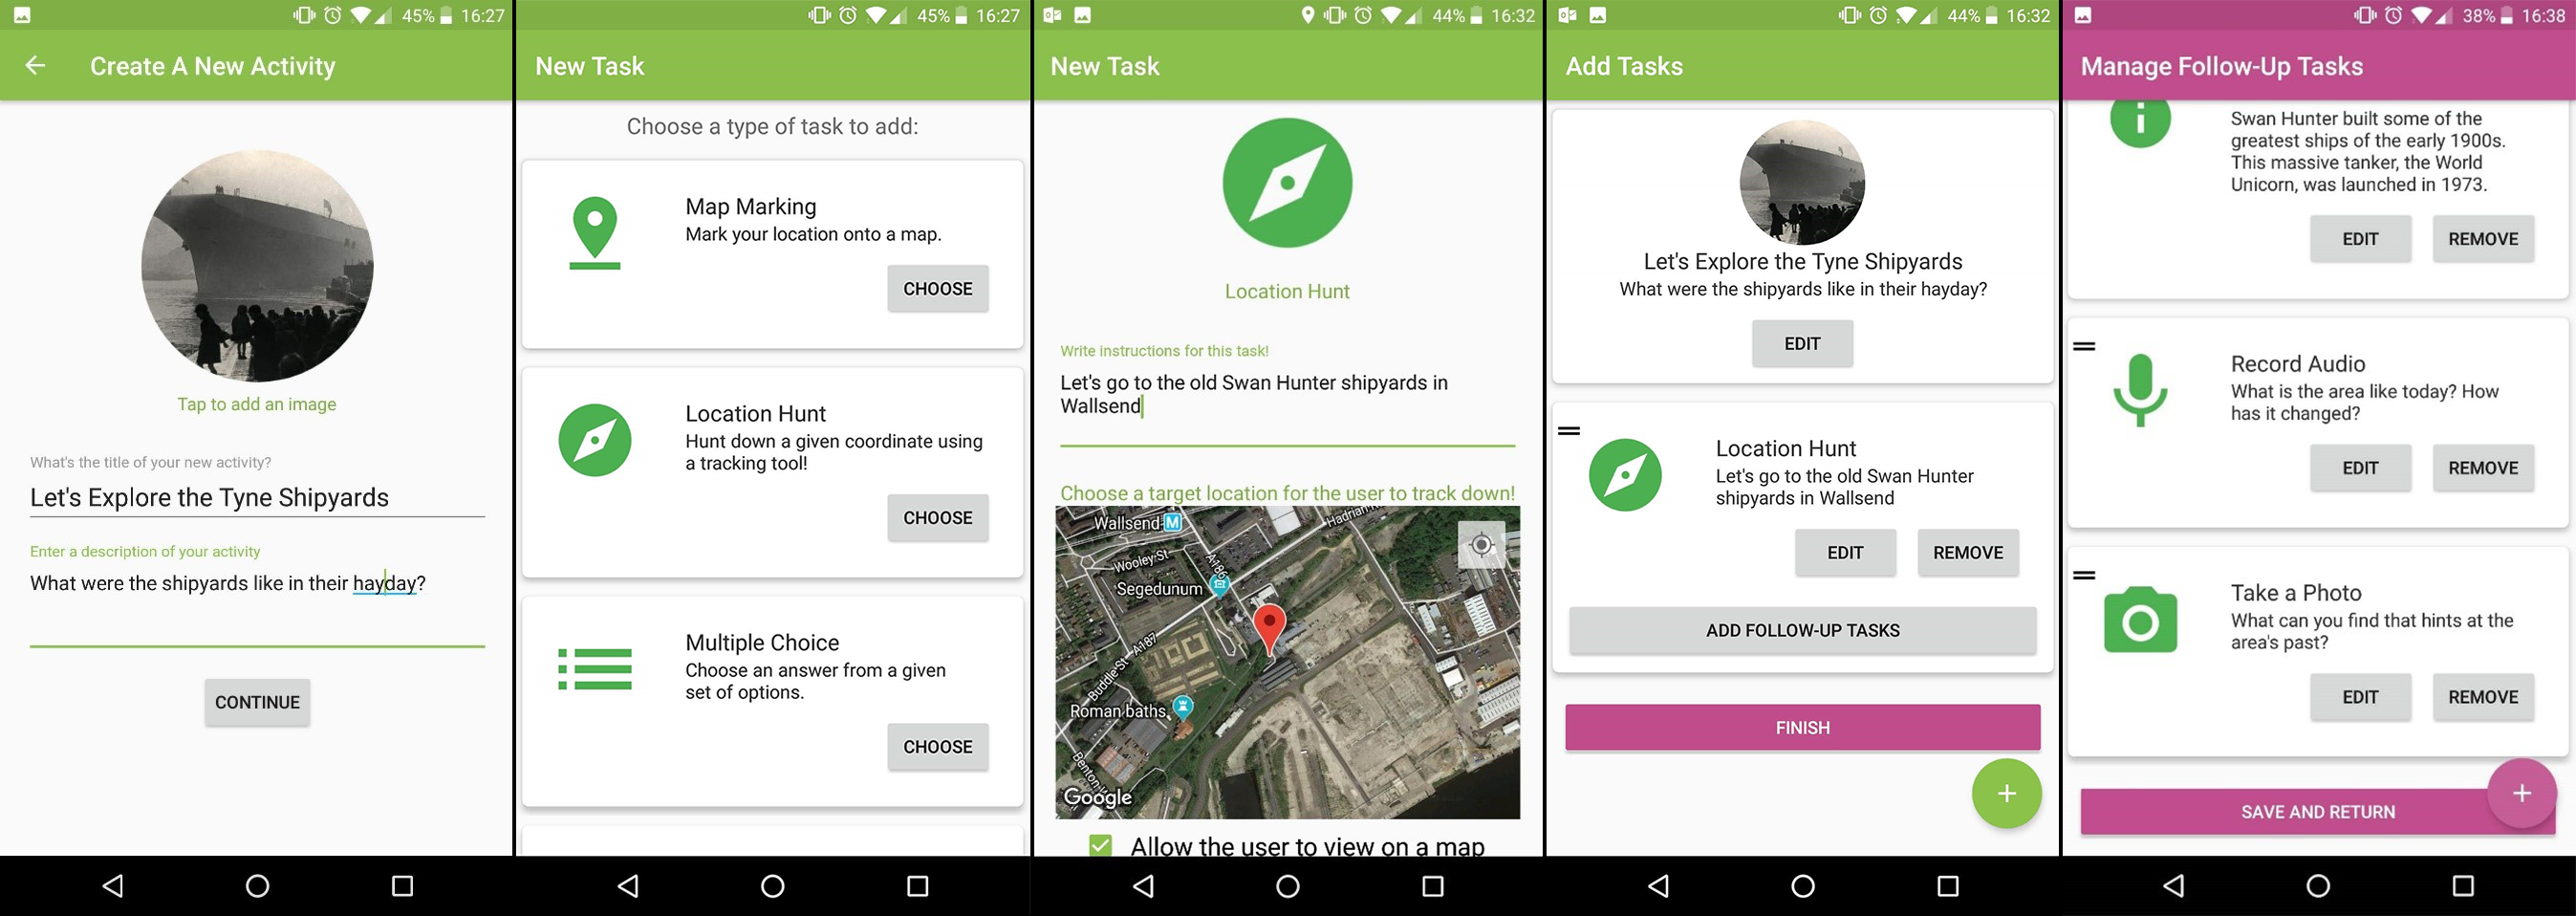
\includegraphics[width=2.1\columnwidth]{figures/activityCreation}
  \caption{Creating an OurPlace activity (left to right): a) Choosing the activity's title, description and image; b) Choosing a Task Type to add; c) Adding a \textit{Location Hunt} Task, with description and target coordinates; d) The new Task in the Activity; e) Adding Follow-Up Tasks to the \textit{Location Hunt}  }~\label{fig:ActivityCreation}
\end{figure*}

Activities are created within the app itself. After supplying a title, description and an optional image (Figure~\ref{fig:ActivityCreation}.a), the designer creates the Tasks that make up the Activity (Figure~\ref{fig:ActivityCreation}.b). Each Task Type requires at least a written instruction for the learner (e.g. A \textit{Location Hunt} might say \textit{`Can you find Carter's Well?'}), but some of them require some additional customization (e.g. supplying geographic coordinates by tapping on a Google Maps view) (Figure~\ref{fig:ActivityCreation}.c). When a Task Type requires an additional file (e.g. a target image for \textit{Photo Match} or an audio recording for \textit{Listen to Audio}), creators are able to either create them through the app itself or load it from an external source (such as Google Drive, Dropbox or files otherwise downloaded from the web). This means that no additional equipment or software is required to create activities (other than \textit{Scan the QR Code}, which requires creators to print the generated QR code from the OurPlace website). Once finished, Activities can be tagged as being relevant to a location before uploading, making it easier for others to find. Additionally, QR codes can be printed from the OurPlace website which launch the activity when scanned in the app.


\section{Overview of the OurPlace Curriculum (IRPCPE)}

\subsection{Introducing the Medium (I)}

\subsection{Researching the Domain (R)}

\subsection{Prototyping (P)}

\subsection{Constructing (C)}

\subsection{Sharing with Peers in the Wild (P)}

\subsection{Sharing Externally in the Wild (E)}

\section{Studies}

\subsection{Study 1: Time-Limited (IR-C--)}

\subsection{Study 2: Without Sharing Externally (IRPCP-)}

\subsection{Study 3: Without Introducing the Medium (-RPC-E)}

\subsection{Planning the Full Curriculum (IRPCPE)}

\section{Findings}

\section{Discussion}

\subsection{Students' Desire for Independence}

\subsection{Focusing on Medium over Domain}

\subsection{Mobile Learning Activities as the Object}
Requires activity theory?

\subsection{Local Heritage as a Learning Resource}

\section{Conclusion}

% Use a numbered list of references at the end of the article, ordered
% alphabetically by first author, and referenced by numbers in
% brackets~\cite{ethics, Klemmer:2002:WSC:503376.503378,
%   Mather:2000:MUT, Zellweger:2001:FAO:504216.504224}. For papers from
% conference proceedings, include the title of the paper and an
% abbreviated name of the conference (e.g., for Interact 2003
% proceedings, use \textit{Proc. Interact 2003}). Do not include the
% location of the conference or the exact date; do include the page
% numbers if available. See the examples of citations at the end of this
% document. Within this template file, use the \texttt{References} style
% for the text of your citation.

% Your references should be published materials accessible to the
% public.  Internal technical reports may be cited only if they are
% easily accessible (i.e., you provide the address for obtaining the
% report within your citation) and may be obtained by any reader for a
% nominal fee.  Proprietary information may not be cited. Private
% communications should be acknowledged in the main text, not referenced
% (e.g., ``[Robertson, personal communication]'').

\section{Quotations}
Quotations may be italicized when \textit{``placed inline''}.

\begin{quote}
Longer quotes, when placed in their own paragraph, need not be
italicized or in quotation marks when indented.  
\end{quote}

\section{Language, Style, and Content}

The written and spoken language of SIGCHI is English. Spelling and
punctuation may use any dialect of English (e.g., British, Canadian,
US, etc.) provided this is done consis- tently. Hyphenation is
optional. To ensure suitability for an international audience, please
pay attention to the following:

\begin{itemize}
\item Write in a straightforward style.
\item Try to avoid long or complex sentence structures.
\item Use common and basic vocabulary (e.g., use the word ``unusual'' rather than the word ``arcane''.
\item Briefly define or explain all technical terms that may be
  unfamiliar to readers.
\item Explain all acronyms the first time they are used in your
  text---e.g., ``Digital Signal Processing (DSP)''.
\item Explain local references (e.g., not everyone knows all city
  names in a particular country).
\item Explain ``insider'' comments. Ensure that your whole audience
  understands any reference whose meaning you do not describe (e.g.,
  do not assume that everyone has used a Macintosh or a particular
  application).
\item Explain colloquial language and puns. Understanding phrases like
  ``red herring'' may require a local knowledge of English.  Humor and
  irony are difficult to translate.
\item Use unambiguous forms for culturally localized concepts, such as
  times, dates, currencies, and numbers (e.g., ``1--5--97'' or
  ``5/1/97'' may mean 5 January or 1 May, and ``seven o'clock'' may
  mean 7:00 am or 19:00). For currencies, indicate equivalences:
  ``Participants were paid {\fontfamily{txr}\selectfont \textwon}
  25,000, or roughly US \$22.''
\item Be careful with the use of gender-specific pronouns (he, she)
  and other gendered words (chairman, manpower, man-months). Use
  inclusive language that is gender-neutral (e.g., she or he, they,
  s/he, chair, staff, staff-hours, person-years). See the
  \textit{Guidelines for Bias-Free Writing} for further advice and
  examples regarding gender and other personal
  attributes~. Be particularly aware of
  considerations around writing about people with disabilities.
\item If possible, use the full (extended) alphabetic character set
  for names of persons, institutions, and places (e.g.,
  Gr{\o}nb{\ae}k, Lafreni\'ere, S\'anchez, Nguy{\~{\^{e}}}n,
  Universit{\"a}t, Wei{\ss}enbach, Z{\"u}llighoven, \r{A}rhus, etc.).
  These characters are already included in most versions and variants
  of Times, Helvetica, and Arial fonts.
\end{itemize}

\section{Accessibility}
The Executive Council of SIGCHI has committed to making SIGCHI
conferences more inclusive for researchers, practitioners, and
educators with disabilities. As a part of this goal, the all authors
are asked to work on improving the accessibility of their
submissions. Specifically, we encourage authors to carry out the
following five steps:
\begin{enumerate}
\item Add alternative text to all figures
\item Mark table headings
\item Add tags to the PDF
\item Verify the default language
\item Set the tab order to ``Use Document Structure''
\end{enumerate}
For more information and links to instructions and resources, please
see: \url{http://chi2016.acm.org/accessibility}.  The
\texttt{{\textbackslash}hyperref} package allows you to create well tagged PDF files,
please see the preamble of this template for an example.

\section{Page Numbering, Headers and Footers}
Your final submission should not contain footer or header information
at the top or bottom of each page. Specifically, your final submission
should not include page numbers. Initial submissions may include page
numbers, but these must be removed for camera-ready. Page numbers will
be added to the PDF when the proceedings are assembled.

\section{Producing and Testing PDF Files}

We recommend that you produce a PDF version of your submission well
before the final deadline.  Your PDF file must be ACM DL
Compliant. The requirements for an ACM Compliant PDF are available at:
{\url{http://www.scomminc.com/pp/acmsig/ACM-DL-pdfs-requirements.htm}}.

Test your PDF file by viewing or printing it with the same software we
will use when we receive it, Adobe Acrobat Reader Version 10. This is
widely available at no cost. Note that most
reviewers will use a North American/European version of Acrobat
reader, so please check your PDF accordingly.

\section{Conclusion}

It is important that you write for the SIGCHI audience. Please read
previous years' proceedings to understand the writing style and
conventions that successful authors have used. It is particularly
important that you state clearly what you have done, not merely what
you plan to do, and explain how your work is different from previously
published work, i.e., the unique contribution that your work makes to
the field. Please consider what the reader will learn from your
submission, and how they will find your work useful. If you write with
these questions in mind, your work is more likely to be successful,
both in being accepted into the conference, and in influencing the
work of our field.

\section{Acknowledgments}

Sample text: We thank all the volunteers, and all publications support
and staff, who wrote and provided helpful comments on previous
versions of this document. Authors 1, 2, and 3 gratefully acknowledge
the grant from NSF (\#1234--2012--ABC). \textit{This whole paragraph is
  just an example.}

% Balancing columns in a ref list is a bit of a pain because you
% either use a hack like flushend or balance, or manually insert
% a column break.  http://www.tex.ac.uk/cgi-bin/texfaq2html?label=balance
% multicols doesn't work because we're already in two-column mode,
% and flushend isn't awesome, so I choose balance.  See this
% for more info: http://cs.brown.edu/system/software/latex/doc/balance.pdf
%
% Note that in a perfect world balance wants to be in the first
% column of the last page.
%
% If balance doesn't work for you, you can remove that and
% hard-code a column break into the bbl file right before you
% submit:
%
% http://stackoverflow.com/questions/2149854/how-to-manually-equalize-columns-
% in-an-ieee-paper-if-using-bibtex
%
% Or, just remove \balance and give up on balancing the last page.
%
\balance{}

\section{References Format}
Your references should be published materials accessible to the
public. Internal technical reports may be cited only if they are
easily accessible and may be obtained by any reader for a nominal
fee. Proprietary information may not be cited. Private communications
should be acknowledged in the main text, not referenced (e.g.,
[Golovchinsky, personal communication]). References must be the same
font size as other body text. References should be in alphabetical
order by last name of first author. Use a numbered list of references
at the end of the article, ordered alphabetically by last name of
first author, and referenced by numbers in brackets. For papers from
conference proceedings, include the title of the paper and the name of
the conference. Do not include the location of the conference or the
exact date; do include the page numbers if available. 

References should be in ACM citation format:
\url{http://www.acm.org/publications/submissions/latex_style}.  This
includes citations to Internet
resources~\cite{CHINOSAUR:venue,cavender:writing,psy:gangnam}
according to ACM format, although it is often appropriate to include
URLs directly in the text, as above. Example reference formatting for
individual journal articles~\cite{ethics}, articles in conference
proceedings~\cite{Klemmer:2002:WSC:503376.503378},
books~\cite{Schwartz:1995:GBF}, theses~\cite{sutherland:sketchpad},
book chapters~\cite{winner:politics}, an entire journal
issue~\cite{kaye:puc},
websites~\cite{acm_categories,cavender:writing},
tweets~\cite{CHINOSAUR:venue}, patents~\cite{heilig:sensorama}, 
games~\cite{supermetroid:snes}, and
online videos~\cite{psy:gangnam} is given here.  See the examples of
citations at the end of this document and in the accompanying
\texttt{BibTeX} document. This formatting is a edited version of the
format automatically generated by the ACM Digital Library
(\url{http://dl.acm.org}) as ``ACM Ref.'' DOI and/or URL links are
optional but encouraged as are full first names. Note that the
Hyperlink style used throughout this document uses blue links;
however, URLs in the references section may optionally appear in
black.

% BALANCE COLUMNS
\balance{}

% REFERENCES FORMAT
% References must be the same font size as other body text.
\bibliographystyle{SIGCHI-Reference-Format}
\bibliography{sample}

\end{document}

%%% Local Variables:
%%% mode: latex
%%% TeX-master: t
%%% End:
